\begin{center}
	\textbf{Đề kiểm tra số 1}
\end{center}
\Opensolutionfile{ans}[ans/ansCD2D1-7DKt1]
\begin{ex}%[2D1Y1-1]%Câu 1.
	Cho hàm số $y=\dfrac{2x+1}{1-x}$. Mệnh đề nào sau đây đúng?
	\choice
	{Hàm số nghịch biến trên $(-\infty; 1)$ và $(1;+\infty)$}
	{Hàm số đồng biến trên $\mathbb{R}\setminus\{1\}$}
	{\True Hàm số đồng biến trên $(-\infty; 1)$ và $(1;+\infty)$}
	{Hàm số đồng biến trên $(-\infty; 1)\cup(1;+\infty)$}
	\loigiai{
		Tập xác định $\mathscr{D}=\mathbb{R}\setminus\{1\}$.\\ Ta có  $y'=\dfrac{3}{(-x+1)^2}>0$, $\forall x\in \mathscr{D}$.\\
		Vậy hàm số đồng biến trên $(-\infty; 1)$ và $(1;+\infty)$.}
\end{ex}
\begin{ex}%[2D1Y4-1]%Câu 2.
	Đường thẳng $y=-1$ là tiệm cận ngang của đồ thị hàm số nào sau đây?
	\choice
	{$y=\dfrac{1+x^2}{1+x}$}
	{$y=\dfrac{2x^2+3x+2}{2-x}$}
	{$y=\dfrac{2x-2}{x+2}$}
	{\True $y=\dfrac{1+x}{1-x}$}
	\loigiai{
		Ta có $\lim\limits_{x\to+\infty}\dfrac{1+x}{1-x}=-1$. Suy ra $y=-1$ là tiệm cận ngang của đồ thị hàm số $y=\dfrac{1+x}{1-x}$.}
\end{ex}
\begin{ex}%[2D1B5-1]%Câu 3.
	Bảng biến thiên sau là bảng biến thiên của hàm số nào sau đây?
	\begin{center}
		
\begin{tikzpicture}[scale=1, font=\footnotesize, line join=round, line cap=round, >=stealth]
		\tkzTab[nocadre=false,lgt=1.2,espcl=2.5,deltacl=0.6]
		{$x$/.6, $y'$/.6, $y$/2.0} % cột đầu tiên
		{$-\infty$, $0$, $2$, $+\infty$} % hàng 1 cột 2
		{,-,0,+,0,-,} % hàng 2 cột 2
		{+/ $+\infty$, -/ $-2$, +/ $2$ , -/ $-\infty$} % hàng 3 cột 2
		\end{tikzpicture}
	\end{center}
	\choice
	{$y=x^3-3x^2-1$}
	{\True $y=-x^3+3x^2-2$}
	{ $y=-x^3+3x^2-1$}
	{$y=-x^3-3x-2$}
	\loigiai{
		Vì $\lim\limits_{x\to-\infty} y=+\infty$ nên hệ số của $x^3$ phải âm $\Rightarrow$ loại $y=x^3-3x^2-1$.\\
		Tại $x=0$ thì $y=-2$ $\Rightarrow$ loại $y=-x^3+3x^2-1$.\\
		$y'=0$ có hai nghiệm phân biệt$\Rightarrow$ loại $y=-x^3-3x-2$.\\
		Vậy $y=-x^3+3x^2-2$
		}
\end{ex}
\begin{ex}%[2D1Y3-1]%Câu 4.
	Hàm số $y=f(x)$ liên tục và có bảng biến thiên trong đoạn $[-1; 3]$ cho trong hình bên. Gọi $M$ là giá trị lớn nhất của hàm số $y=f(x)$ trên đoạn $[-1;3]$. Tìm mệnh đề đúng?
	\begin{center}
		
\begin{tikzpicture}[scale=1, font=\footnotesize, line join=round, line cap=round, >=stealth]
		\tkzTab[nocadre=false,lgt=1.2,espcl=2.5,deltacl=0.6]
		{$x$/.6, $f’(x)$/.6, $f(x)$/2.0} % cột đầu tiên
		{$-1$, $0$, $2$, $3$} % hàng 1 cột 2
		{,+,0,-,0,+,} % hàng 2 cột 2
		{-/ $0$, +/ $5$, -/ $1$ , +/ $4$} % hàng 3 cột 2
		\end{tikzpicture}
	\end{center}
	
	\choice
	{$M=f(-1)$}
	{$M=f(3)$}
	{$M=f(2)$}
	{\True $M=f(0)$}
	\loigiai{
		Dựa vào bảng biến thiên, ta có $M=f(0)$.}
\end{ex}
\begin{ex}%[2D1Y2-2]%Câu 5.
	Cho hàm số $y=f(x)$ có bảng biến thiên như hình bên: 
	\begin{center}
		
\begin{tikzpicture}[scale=1, font=\footnotesize, line join=round, line cap=round, >=stealth]
		\tkzTab[nocadre=false,lgt=1.2,espcl=2.5,deltacl=0.6]
		{$x$/.6, $f’(x)$/.6, $f(x)$/2.0} % cột đầu tiên
		{$-\infty$, $2$, $4$, $+\infty$} % hàng 1 cột 2
		{,+,0,-,0,+,} % hàng 2 cột 2
		{-/ $-\infty$, +/ $3$, -/ $-2$ , +/ $+\infty$} % hàng 3 cột 2
		\end{tikzpicture}
	\end{center}
	Khẳng định nào sau đây là đúng?
	\choice
	{Hàm số đạt cực đại tại $x=3$}
	{Hàm số đạt cực đại tại $x=4$}
	{\True Hàm số đạt cực đại tại $x=2$}
	{Hàm số đạt cực đại tại $x=-2$}
	\loigiai{
		Giá trị cực đại của hàm số là $y=3$ tại $x=2$.}
\end{ex}
\begin{ex}%[2D1Y1-2]%Câu 6.
	Cho đồ thị hàm số như hình vẽ. 
\begin{center}
	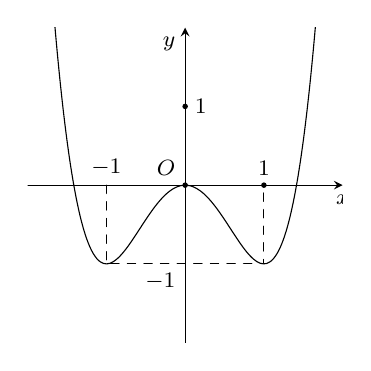
\begin{tikzpicture}[scale=1, font=\footnotesize, line join=round, line cap=round, >=stealth]
	\def \f(#1){((#1)^4-2*(#1)^2)/1}
	\clip(-2,-2) rectangle (2,2)  ; % vùng lấy hình
	\draw[->] (-2,0) -- (2,0) node[below]{ $x$};
	\draw[->] (0,-2) -- (0,2) node[below left]{ $y$};
	\draw[smooth,samples=100,domain=-2.1:2.1] plot(\x,{\f(\x)});
	\draw[dashed] (-1,0) node[above]{$-1$}--(-1,-1)--(0,-1)node[below left] {$-1$} --(1,-1)--(1,0);
	\fill (0,0) node[above left] {$O$} circle (1pt) (1,0) node[above] {$1$} circle (1pt) (0,1) node[right] {$1$} circle (1pt)
	(0,3) node[left] {$3$} circle (1pt) (0,5) node[left] {$5$} circle (1pt) ;
	
	\end{tikzpicture}
\end{center}
	Mệnh đề nào dưới đây đúng?
	\choice
	{Hàm số luôn đồng biến trên $\mathbb{R}$}
	{Hàm số nghịch biến trên $(1;+\infty)$}
	{Hàm số đồng biến trên $(-1;+\infty)$}
	{\True Hàm số nghịch biến trên $(-\infty;-1)$}
	\loigiai{
		Dựa vào đồ thị ta thấy hàm số nghịch biến trên $(-\infty;-1)$.}
\end{ex}
\begin{ex}%[2D1B5-4]%Câu 7.
	Cho hàm số $y=x^4-4x^2-2$ có đồ thị $(C)$ và đồ thị $(P)$: $y=1-x^2$. Số giao điểm của $(P)$ và đồ thị $(C)$ là
	\choice
	{$1$}
	{$4$}
	{\True $2$}
	{$3$}
	\loigiai{
		Phương trình hoành độ giao điểm của $(P)$ và $(C)$: $x^4-4x^2-2=1-x^2\Leftrightarrow x^4-3x^2-3=0. \quad (1)$ \\
		Đặt $t=x^2$ ta được phương trình trung gian: $t^2-3t-3=0. \quad (2)$\\
		Vì $(2)$ có hai nghiệm phân biệt trái dấu nên $(1)$ sẽ có hai nghiệm phân biệt.\\
		Vậy số giao điểm của $(P)$ và đồ thị $(C)$ là $2$ giao điểm.}
\end{ex}
\begin{ex}%[2D1K3-1]%Câu 8.
	Biết rằng giá trị lớn nhất của hàm số $y=x+\sqrt{4-x^2}+m$ là $3\sqrt{2}$. Giá trị của $m$ là
	\choice
	{\True $m=\sqrt{2}$}
	{$m=2\sqrt{2}$}
	{$m=\dfrac{\sqrt{2}}{2}$}
	{$m=-\sqrt{2}$}
	\loigiai{
		Tập xác định $\mathscr{D}=[-2; 2]$.\\
		$y'=1-\dfrac{x}{\sqrt{4-x^2}};\ y=0\Leftrightarrow\sqrt{4-x^2}-x=0\Leftrightarrow\heva{&x\geq 0\\&4-x^2=x^2}\Leftrightarrow\heva{&x\geq 0\\&x=\pm\sqrt{2}}\Leftrightarrow x=\sqrt{2.}$ \\
		$f(2)=2+m$; $f(-2)=-2+m$; $f(\sqrt{2})=2\sqrt{2}+m$.
		Nên giá trị lớn nhất của hàm số là $2\sqrt{2}+m$.\\
		Ta có $2\sqrt{2}+m=3\sqrt{2}\Leftrightarrow m=\sqrt{2}$.}
\end{ex}
\begin{ex}%[2D1B4-2]%Câu 9.
	Tìm tất cả các giá trị của tham số $m$ để đồ thị hàm số $y=\dfrac{2x+4}{x-m}$ có tiệm cận đứng. 
	\choice
	{\True $m\neq-2$}
	{$m >-2$}
	{$m=-2$}
	{$m <-2$}
	\loigiai{
		Yêu cầu bài toán $\Leftrightarrow$ Phương trình $x-m=0$ có nghiệm khác $-2\Rightarrow m\neq-2$.}
\end{ex}
\begin{ex}%[2D1G1-3]%Câu 10.
	Tìm tất cả các giá trị thực của tham số $m$ để hàm số $y=mx-\sin x$ đồng biến trên $\mathbb{R}$. 
	\choice
	{$m>1$}
	{$m\leq-1$}
	{\True $m\geq 1$}
	{$m\geq-1$}
	\loigiai{
		TXĐ: $\mathscr{D}=\mathbb{R}$.\\
		$y'=m-\cos x$.\\
		Hàm số đồng biến trên $\mathbb{R}\Leftrightarrow y'\geq 0,\forall x\in\mathbb{R}\Leftrightarrow m\geq\sin x,\forall x\in\mathbb{R}\Leftrightarrow m\geq 1$.}
\end{ex}
\begin{ex}%[2D1K5-3]%Câu 11.
	Tìm tất các các giá trị thực của tham số $m$ để phương trình $x^3-3x+2m=0$ có ba nghiệm thực phân biệt. 
	\choice
	{$m\in(-2;2)$}
	{\True $m\in(-1;1)$}
	{$m\in(-\infty;-1)\cup(1;+\infty)$}
	{$m\in(-2;+\infty)$}
	\loigiai{
		Ta có: $x^3-3x+2m=0\Leftrightarrow-x^3+3x=2m \quad (*)$.\\
		Xét hàm số $y=-x^3+3x$ có đồ thị là $(C)$ và đường thẳng $d\colon y=2m$.\\
		Số nghiệm của phương trình $(*)$ phụ thuộc vào số giao điểm của đồ thị hàm số $(C)$ và đường thẳng $d$.\\
		Ta có: $y'=-3x^2+3$, cho $y'=0\Leftrightarrow-3x^2+3=0\Leftrightarrow\hoac{&x=-1\\&x=1.}$ \\
		Bảng biến thiên
		\begin{center}
			
\begin{tikzpicture}[scale=1, font=\footnotesize, line join=round, line cap=round, >=stealth]
			\tkzTab[nocadre=false,lgt=1.2,espcl=2.5,deltacl=0.6]
			{$x$/.6, $f’(x)$/.6, $f(x)$/2.0} % cột đầu tiên
			{$-\infty$, $-1$, $1$, $+\infty$} % hàng 1 cột 2
			{,-,0,+,0,-,} % hàng 2 cột 2
			{+/ $+\infty$, -/ $-2$, +/ $2$ , -/ $-\infty$} % hàng 3 cột 2
			\end{tikzpicture}
		\end{center}
		Từ bảng biến thiên thì phương trình $(*)$ có ba nghiệm phân biệt khi $-2<2m<2\Leftrightarrow-1<m<1$.}
\end{ex}
\begin{ex}%[2D1B2-1]%Câu 12.
	PTĐT đi qua hai điểm cực trị của đồ thị hàm số $y=x^3-6x^2+9x-2$ là
	\choice
	{$y=2x+4$}
	{$y=-x+2$}
	{$y=2x-4$}
	{\True $y=-2x+4$}
	\loigiai{
		Ta có: $y'=3x^2-12x+9$, cho $y'=0\Rightarrow 3x^2-12x+9=0\Rightarrow\hoac{&x=1\\&x=3}$ 
		\begin{center}
			
\begin{tikzpicture}[scale=1, font=\footnotesize, line join=round, line cap=round, >=stealth]
			\tkzTab[nocadre=false,lgt=1.2,espcl=2.5,deltacl=0.6]
			{$x$/.6, $f’(x)$/.6, $f(x)$/2.0} % cột đầu tiên
			{$-\infty$, $1$, $3$, $+\infty$} % hàng 1 cột 2
			{,+,0,-,0,+,} % hàng 2 cột 2
			{-/ $-\infty$, +/ $2$, -/ $-2$ , +/ $+\infty$} % hàng 3 cột 2
			\end{tikzpicture}
		\end{center}
		Đồ thị hàm số đạt cực trị tại $A(1;2)$ và $B(3;-2)$.\\
		Suy ra đường thẳng đi qua hai điểm cực trị là $y=-2x+4$.}
\end{ex}
\begin{ex}%[2D1B1-2]%Câu 13.
	Cho hàm số $y=f(x)$ liên tục trên $\mathbb{R}$ và có đạo hàm $f'(x)=(x+1)^2(x-1)^3(2-x)$. Hàm số $y=f(x)$ đồng biến trên khoảng nào dưới đây?
	\choice
	{\True $(1;2)$}
	{$(-\infty;-1)$}
	{$(-1;1)$}
	{$(2;+\infty)$}
	\loigiai{
		Ta có $f'(x)=0\Leftrightarrow(x+1)^2(x-1)^3(2-x)=0\Leftrightarrow\hoac{&x=-1\\&x=1\\&x=2.}$ \\
		Lập bảng xét dấu của $f'(x)$ ta được: 
	\begin{center}
		
\begin{tikzpicture}[scale=1]
		\tkzTabInit[nocadre=false, lgt=1.2, espcl=2.5, deltacl=0.6]{$x$/0.6, $f'(x)$/0.6}{$-\infty$, $-1$, $1$, $2$, $+\infty$}
		\tkzTabLine{,-,0,-,0,+,0,-,}
		\end{tikzpicture}	
	\end{center}
		Vậy hàm số $y=f(x)$ đồng biến trên khoảng $(1;2)$.}
\end{ex}
\begin{ex}%[2D1B2-1]%Câu 14.
	Đồ thị của hàm số $y=-x^3+3x^2+9x+1$ có hai điểm cực trị $A$ và $B$. Điểm nào dưới đây thuộc đường thẳng $AB$?
	\choice
	{\True $N(1; 12)$}
	{$M(1;-12)$}
	{$\mathrm{P}(1; 0)$}
	{$Q(0;-1)$}
	\loigiai{
		Tập xác định $\mathbb{R}$.\\
		$y'=-3x^2+6x+9$.\\
		$y'=0\Leftrightarrow-3x^2+6x+9=0\Leftrightarrow\hoac{&x=-1\\&x=3.}$ \\
		Do đó đồ thị hàm số có hai điểm cực trị là $A(-1;-4)$ và $B(3;28)$.\\
		Suy ra đường thẳng $AB$ có phương trình $8x-y+4=0$.\\
		Thay $N(1; 12)$ vào phương trình $AB$ ta có $8.1-12+4=0$. Vậy $N$ thuộc $AB$.}
\end{ex}
\begin{ex}%[2D1G3-6]%Câu 15.
	Một chất điểm chuyển động theo quy luật $s(t)=-t^3+6t^2$ với $t$ là thời gian tính từ lúc bắt đầu chuyển động, $s(t)$ là quãng đường đi được trong khoảng thời gian $t$. Tính thời điểm $t$ tại đó vận tốc đạt giá trị lớn nhất. 
	\choice
	{$t=3$}
	{$t=4$}
	{$t=1$}
	{\True $t=2$}
	\loigiai{
		Ta có $v(t)=s'(t)=-3t^2+12t$ có đồ thị là Parabol, do đó $v(t)_{\max}\Leftrightarrow t=\dfrac{-12}{-6}=2$.}
\end{ex}
\begin{ex}%[2D1K5-7]%Câu 16.
	Trên đồ thị $(C)$ của hàm số $y=\dfrac{x+10}{x+1}$ có bao nhiêu điểm có tọa độ nguyên?
	\choice
	{$4$}
	{$2$}
	{$10$}
	{\True $6$}
	\loigiai{
		Ta có $y=\dfrac{x+10}{x+1}=1+\dfrac{9}{x+1}$.\\
		Điểm trên đồ thị hàm số có tọa độ nguyên nghĩa là $x\in\mathbb{Z};y\in\mathbb{Z}$.\\
		Để $y\in\mathbb{Z}\Rightarrow 9\vdots(x+1)\Rightarrow\hoac{&x+1=\pm 1\\&x+1=\pm 3\\&x+1=\pm 9.}$ \\
		Vậy trên đồ thị hàm số có 6 điểm có tọa độ nguyên.}
\end{ex}
\begin{ex}%[2D1K5-4]%Câu 17.
	Cho hàm số $y=\dfrac{2x-1}{x+1}$ có đồ thị $(C)$ và đường thẳng $d\colon y=2x-3$. Đường thằng $d$ cắt $(C)$ tại hai điểm $A$ và $B$. Khoảng cách giữa $A$ và $B$ là
	\choice
	{$AB=\dfrac{2\sqrt{5}}{5}$}
	{$AB=\dfrac{5}{2}$}
	{\True $AB=\dfrac{5\sqrt{5}}{2}$}
	{$AB=\dfrac{2}{5}$}
	\loigiai{
		Phương trình hoành độ giao điểm của đồ thị $(C)$ và đường thẳng $d$:\\
		$\dfrac{2x-1}{x+1}=2x-3\Leftrightarrow\heva{&x\neq-1\\&2x^2-3x-2=0}\Leftrightarrow\hoac{&x=2\Rightarrow y=1\\&x=-\dfrac{1}{2}\Rightarrow y=-4}\Rightarrow A(2;1)$, $B\left(-\dfrac{1}{2};-4\right)$.\\
		Ta có $\overrightarrow{AB}=\left(-\dfrac{5}{2};-5\right)$. Suy ra $AB=\dfrac{5\sqrt{5}}{2}$.}
\end{ex}
\begin{ex}%[2D1G5-4]%Câu 18.
	Tìm giá trị thực của tham số $m$ để đồ thị hàm số $y=x^3-3x^2+2$ cắt đường thẳng $d\colon y=m(x-1)$ tại ba điểm phân biệt có hoành độ $x_1,x_2,x_3$ thỏa mãn $x_1^2+x_2^2+x_3^2>5$. 
	\choice
	{$m\geq-3$}
	{$m\geq-2$}
	{$m >-3$}
	{\True $m >-2$}
	\loigiai{
		PT hoành độ giao điểm: $x^3-3x^2+2=m(x-1)$ \\
		$ \Leftrightarrow(x-1)\left(x^2-2x-2-m\right)=0\Leftrightarrow\hoac{&x_1=1\\&x^2-2x-2-m=0.\quad (1)} $ \\
		Yêu cầu bài toán $\Leftrightarrow (1)$ có hai nghiệm phân biệt $x_2,x_3$ khác $x_1=1$ và thỏa mãn $1+x_2^2+x_3^2>5$ \\
		$ \Leftrightarrow\heva{&\Delta'=m+3>0\\&1-2-2-m\neq 0\\&1+S^2-2P>5}\Leftrightarrow\heva{&m+3>0\\&-3-m\neq 0\\&1+4+4+2m>5}\Leftrightarrow m >-2 $.}
\end{ex}
\begin{ex}%[2D1G4-1]%Câu 19.
	Tìm tổng số đường tiệm cận ngang và tiệm cận đứng của đồ thị hàm số $y=\dfrac{x-1}{4\sqrt{3x+1}-3x-5}$ 
	\choice
	{$3$}
	{$0$}
	{$1$}
	{\True $2$}
	\loigiai{
		Ta có $4\sqrt{3x+1}-3x-5=0\Leftrightarrow 4\sqrt{3x+1}=3x+5$ \\
		$ \Leftrightarrow\heva{&3x+5\geq 0\\&16(3x+1)=(3x+5)^2}\Leftrightarrow\heva{&x\geq-\dfrac{5}{3}\\&9x^2-18x+9=0}\Leftrightarrow x=1 $.\\
		TXĐ: $\mathscr{D}=\left[-\dfrac{1}{3};+\infty\right)\setminus\{1\}$.\\
		Ta có $\lim\limits_{x\to 1^-} y=\lim\limits_{x\to 1^-}\dfrac{(x-1)\left(4\sqrt{3x+1}+3x+5\right)}{-9(x-1)^2} =\lim\limits_{x\to 1^-}\dfrac{4\sqrt{3x+1}+3x+5}{-9(x-1)}=+\infty$.\\
		$\Rightarrow$ đồ thị hàm số có $1$ đường tiệm cận đứng là $x=1$.\\
		Ta có $\lim\limits_{x\to+\infty} y=\lim\limits_{x\to+\infty}\dfrac{x-1}{4\sqrt{3x+1}-3x-5}=-\dfrac{1}{3}$.\\
		$\Rightarrow$ đồ thị hàm số có $1$ đường tiệm cận ngang là $y=-\dfrac{1}{3}$.\\
		Vậy tổng số tiệm cận đứng và tiệm cận ngang của đồ thị hàm số là $2$.}
\end{ex}
\begin{ex}%[2D1G3-6]%Câu 20.
	Người ta cần xây một bể chứa nước sản xuất dạng khối hộp chữ nhật không nắp có thể tích bằng $200$ m$^3$. Đáy bể là hình chữ nhật có chiều dài gấp đôi chiều rộng. Chi phí để xây bể là $300$ nghìn đồng/m$^2$ (chi phí được tính theo diện tích xây dựng, bao gồm diện tích đáy và diện tích xung quanh, không tính chiều dày của đáy và thành bể). Hãy xác định chi phí thấp nhất để xây bể (làm tròn đến đơn vị triệu đồng). 
	\choice
	{$75$ triệu đồng}
	{\True $51$ triệu đồng}
	{$36$ triệu đồng}
	{$46$ triệu đồng}
	\loigiai{
\begin{center}
		\begin{tikzpicture}[scale=1, font=\footnotesize, line join=round, line cap=round, >=stealth]
	\def \a{4}
	\def \b{1}
	\def \c{2}
	\clip(-2,-2) rectangle (5,5);
	\draw (0,\a)--(\a,\a)--(\a-\b,\a-\c)--(-\b,\a-\c)--(0,\a);
	\draw (\a,\a)--(\a,0)--(\a-\b,-\c)--(-\b,-\c)--(-\b,-\c+\a);
	\draw (\a-\b,\a-\c)--(\a-\b,-\c);
	\draw[dashed] (0,\a)--(0,0)--(\a,0) (0,0)--(-\b,-\c);
	\draw (-\b+2,-\c+0.3) node{$2x$} (-\b-.5,\a-4.3) node{$h$} (-\b/2,-\c/2+0.5) node{$x$};
	\end{tikzpicture}
\end{center}
Gọi $x$ là chiều rộng của đáy, $h$ là chiều cao của bể.\\
		Thể tích của khối hộp chữ nhật không nắp bằng $200$ m$^3$ nên ta có\\
		$V=2x\cdot x\cdot h=200 \Rightarrow h=\dfrac{100}{x^2}$.\\
		Diện tích bể nước cần xây là $S=2x^2+6xh=2x^2+\dfrac{600}{x}=f(x)$.\\
		$f'(x)=4x-\dfrac{600}{x^2}=0\Leftrightarrow x=\sqrt[3]{150}$. Suy ra $\min f(x)=f\left(\sqrt[3]{150}\right)$.\\
		Chi phí thấp nhất để xây bể là $f\left(\sqrt[3]{150}\right) \cdot 300.000\approx 51$ triệu đồng.}
\end{ex}
\begin{ex}%[2D1G1-3]%Câu 21.
	Cho hàm số: $y=-\dfrac{x^3}{3}+(a-1)x^2+(a+3)x-4$. Tìm $a$ để hàm số đồng biến trên khoảng $(0; 3)$. 
	\choice
	{\True $a\geq\dfrac{12}{7}$}
	{$a <-3$}
	{$a\leq-3$}
	{$a>\dfrac{12}{7}$}
	\loigiai{
		Ta có: $y'=-x^2+2(a-1)x+a+3$.\\
		Để hàm số đồng biến trên khoảng $(0; 3)$ thì $y'\geq 0,\forall x\in(0; 3)$.\\
		(Dấu $''=''$ chỉ xảy ra tại hữu hạn điểm trên $(0; 3)$)\\
		$ \Leftrightarrow a\geq\dfrac{x^2+2x-3}{2x+1},\forall x\in(0; 3)\Leftrightarrow a\geq\max\limits_{(0; 3)} f(x) $.\\
		Xét hàm số $f(x)=\dfrac{x^2+2x-3}{2x+1}$ trên khoảng $(0; 3)$.\\
		Ta có $f'(x)=\dfrac{2x^2+2x+8}{(2x+1)^2}=\dfrac{2\left(x+\dfrac{1}{2}\right)^2+\dfrac{15}{2}}{(2x+1)^2}>0,\forall x\in(0; 3)$ \\
		$ \Rightarrow f(x) $ luôn đồng biến trên khoảng $(0; 3)\Rightarrow\max\limits_{(0; 3)} f(x)=f(3)=\dfrac{12}{7}$.\\
		Vậy $m\geq\dfrac{12}{7}$.}
\end{ex}
\begin{ex}%[2D1K2-3]%Câu 22.
	Để hàm số $y=\dfrac{x^2+mx+1}{x+m}$ đạt cực đại tại $x=2$ thì $m$ thuộc khoảng nào?
	\choice
	{$(2; 4)$}
	{$(0; 2)$}
	{\True $(-4;-2)$}
	{$(-2; 0)$}
	\loigiai{
		Tập xác định $\mathscr{D}=\mathbb{R}\setminus\{-m\}$.\\
		$y'=\dfrac{x^2+2mx+m^2-1}{(x+m)^2},\forall x\neq-m$.\\
		Điều kiện cần:\\
		Để hàm số đạt cực đại tại $x=2$ thì $y'(2)=0\Leftrightarrow m^2+4m+3=0\Leftrightarrow\hoac{&m=-1\\&m=-3}\Rightarrow$ loại khoảng A, B.\\
		Điều kiện đủ:\\
		Với $m=-1$, ta có $y'=\dfrac{x^2-2x}{(x-1)^2},\forall x\neq 1$; $y'=0\Leftrightarrow\hoac{&x=2\\&x=0.}$ \\
		Bảng biến thiên
		\begin{center}
			\begin{tikzpicture}
			\tkzTabInit[nocadre=false,lgt=1.2,espcl=2.5,deltacl=0.6]
			{$x$ /.6,$y'$ /.6,$y$ /1.5}
			{$-\infty$,$0$,$1$,$2$,$+\infty$}
			\tkzTabLine{,+,$0$,-,d,-,$0$,+,}
			\tkzTabVar{-/ $-\infty$,+/ CĐ,-D+/$-\infty$ / $+\infty$,-/CT,+/$+\infty$}
			\end{tikzpicture}
		\end{center}
		Dựa vào bảng biến thiên ta thấy hàm số đạt cực tiểu tại $x=2\Rightarrow m=-1$ không thoả mãn ycbt.\\
		Với $m=-3$, ta có $y'=\dfrac{x^2-6x+8}{(x-3)^2},\forall x\neq 3$; $y'=0\Leftrightarrow\hoac{&x=4\\&x=2.}$ \\
		Bảng biến thiên
			\begin{center}
				\begin{tikzpicture}
				\tkzTabInit[nocadre=false,lgt=1.2,espcl=2.5,deltacl=0.6]
				{$x$ /.6,$y'$ /.6,$y$ /1.5}
				{$-\infty$,$2$,$3$,$4$,$+\infty$}
				\tkzTabLine{,+,$0$,-,d,-,$0$,+,}
				\tkzTabVar{-/ $-\infty$,+/ CĐ,-D+/$-\infty$ / $+\infty$,-/CT,+/$+\infty$}
				\end{tikzpicture}
			\end{center}
		Dựa vào bảng biến thiên ta thấy hàm số đạt cực tiểu tại $x=2\Rightarrow m=-3$ thoả mãn ycbt.\\
		Vậy $m=-3\in(-4;-2)$.}
\end{ex}
\begin{ex}%[2D1K5-1]%Câu 23.
	Biết rằng hàm số $y=f(x)=ax^4+bx^2+c$ có đồ thị là đường cong trong hình vẽ bên dưới.\\
\begin{center}
	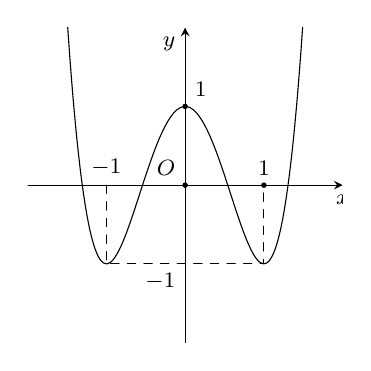
\begin{tikzpicture}[scale=1, font=\footnotesize, line join=round, line cap=round, >=stealth]
	\def \f(#1){(2*(#1)^4-4*(#1)^2+1)/1}
	\clip(-2,-2) rectangle (2,2)  ; % vùng lấy hình
	\draw[->] (-2,0) -- (2,0) node[below]{ $x$};
	\draw[->] (0,-2) -- (0,2) node[below left]{ $y$};
	\draw[smooth,samples=100,domain=-2.1:2.1] plot(\x,{\f(\x)});
	\draw[dashed] (-1,0) node[above]{$-1$}--(-1,-1)--(0,-1)node[below left] {$-1$} --(1,-1)--(1,0);
	\fill (0,0) node[above left] {$O$} circle (1pt) (1,0) node[above] {$1$} circle (1pt) (0,1) node[above right] {$1$} circle (1pt)
	(0,3) node[left] {$3$} circle (1pt) (0,5) node[left] {$5$} circle (1pt) ;
	
	\end{tikzpicture}
\end{center}	
	Tính giá trị $f(a+b+c)$. 
	\choice
	{$f(a+b+c)=-2$}
	{$f(a+b+c)=2$}
	{\True $f(a+b+c)=-1$}
	{$f(a+b+c)=1$}
	\loigiai{
		Ta có $y'=4ax^3+2bx$.\\
		Từ đồ thị, ta có hệ phương trình: $\heva{&f(0)=c=1\\&f'(\pm 1)=2a+b=0\\&f(\pm 1)=a+b+c=-1}\Leftrightarrow\heva{&c=1\\&a=2\\&b=-4.}$ \\
		Suy ra $f(x)=2x^4-4x^2+1\Rightarrow f(a+b+c)=f(-1)=-1$.}
\end{ex}
\begin{ex}%[2D1G5-4]%Câu 24.
	Tìm tất cả các giá trị thực của tham số $m$ để đường thẳng $y=-2x+m$ cắt đồ thị $(H)$ của hàm số $y=\dfrac{2x+3}{x+2}$ tại hai điểm $A, B$ phân biệt sao cho $P=k_1^{2018}+k_2^{2018}$ đạt giá trị nhỏ nhất, với $k_1,k_2$ là hệ số góc của tiếp tuyến tại $A, B$ của đồ thị $(H)$. 
	\choice
	{$m=3$}
	{$m=2$}
	{$m=-3$}
	{\True $m=-2$}
	\loigiai{
		Phương trình hoành độ giao điểm $\dfrac{2x+3}{x+2}=-2x+m$ \\
		$ \Leftrightarrow\heva{&x\neq-2\\&(x+2)(2x-m)+2x+3=0}\Leftrightarrow\heva{&x\neq-2\\&2x^2-(m-6)x+3-2m=0 (1).} $ \\
		Đường thẳng $d\colon y=-2x+m$ cắt $(H)$ tại hai điểm phân biệt\\
		$ \Leftrightarrow $ (1) có 2 nghiệm phân biệt khác $-2\Leftrightarrow\heva{&\Delta=(m-6)^2-8(3-2m)>0\\&2\cdot (-2)^2-(m-6)\cdot (-2)+3-2m\neq 0}$ (*).\\
		Khi đó $x_A, x_B$ là 2 nghiệm phân biệt của (1) $\Rightarrow\heva{&x_A+x_B=\dfrac{m-6}{2}\\&x_Ax_B=\dfrac{3-2m}{2}}$ (2).\\
		Ta có $y'=\dfrac{1}{(x+2)^2}\Rightarrow k_1=\dfrac{1}{(x_A+2)^2}, k_2=\dfrac{1}{(x_B+2)^2}$ \\
		$ \Rightarrow k_1k_2=\dfrac{1}{\left[2(x_A+x_B)+x_Ax_B+4\right]^2}=\dfrac{1}{\left(m-6+\dfrac{3-2m}{2}+4\right)^2}=4 $ \\
		$ \Rightarrow P=k_1^{2018}+k_2^{2018}\geq 2\sqrt{k_1^{2018}k_2^{2018}}=2\sqrt{4^{2018}} $.\\
		Dấu xảy ra $\Leftrightarrow k_1=k_2>0\Leftrightarrow\dfrac{1}{(x_A+2)^2}=\dfrac{1}{(x_B+2)^2}\Leftrightarrow\hoac{&x_A+2=x_B+2\\&x_A+2=-(x_B+2)}$ (3).\\
		Do $\heva{&A\neq B\\&A, B\in(H)}\Rightarrow x_A\neq x_B$ nên (3) $\Leftrightarrow x_A+x_B=-4$.\\
		Kết hợp với (2) ta được $\dfrac{m-6}{2}=-4\Leftrightarrow m=-2$ thỏa mãn (*).}
\end{ex}
\begin{ex}%[2D1G3-5]%Câu 25.
	Cho các số thực dương $x$, $y$. Tìm giá trị lớn nhất của biểu thức $P=\dfrac{4xy^2}{\left(x+\sqrt{x^2+4y^2}\right)^3}$.
	\choice
	{$\max P=1$}
	{$\max P=\dfrac{1}{10}$}
	{\True $\max P=\dfrac{1}{8}$}
	{$\max P=\dfrac{1}{2}$}
	\loigiai{
		$P=\dfrac{4xy^2}{\left(x+\sqrt{x^2+4y^2}\right)^3}=\dfrac{4\left(\dfrac{y}{x}\right)^2}{\left(1+\sqrt{1+4{\left(\dfrac{y}{x}\right)^2}}\right)^3}\left(\forall x>,y>0\right)$.\\
		Đặt $t=\sqrt{1+4\left(\dfrac{y}{x}\right)^2}$, $t>1$. Khi đó biểu thức trở thành $P(t)=\dfrac{t^2-1}{(t+1)^3}$ với $t>1$.\\
		$P'(t)=\dfrac{-t^2+2t+3}{(t+1)^4}=0\Leftrightarrow t=3$.\\
		Bảng biến thiên: 
		\begin{center}
			
\begin{tikzpicture}
			\tkzTabInit[nocadre=false,lgt=1.2,espcl=2.5,deltacl=0.4]
			{$t$ /.6,$P'(t)$ /.6,$P(t)$ /1.5}
			{$1$,$3$,$+\infty$}
			\tkzTabLine{d,+,$0$,-,}
			\tkzTabVar{D-/,+/ $\dfrac{1}{8}$,-/}
			\end{tikzpicture}
		\end{center}
		Vậy $\max P=P(3)=\dfrac{1}{8}$.}
\end{ex}

\Closesolutionfile{ans}
\DAPAN
\inputansbox{10}{ans/ansCD2D1-7DKt1}
%\begin{indapan}
%	{10}{ans/ansCD2D1-7DKt1}
%\end{indapan}


